\chapter{Design} % possible chapter for Projects
\label{chap:design}

This chapter describes the design choices and the overall architecture of the framework. \todo{Expand the introduction}

\section{Framework architecture}
\label{sec:arch-design}

The framework is articulated in modules: each module takes into account a specific aspect of the pulverization.
The modularity of the framework enables from one side, the possibility to use only the needed modules, preventing the bloating of the project;
on the other side, modularity allows the customization of some implementations of the framework.

The two fundamentals modules of the pulverization framework are: \emph{core} and \emph{platform} which respectively define the core concepts
of pulverization like the type of components and all the logic needed to run the pulverized system like defining the components reference,
loading the user-defined components and setup the communications between all of them.

The third module is \emph{rabbitmq-platform} which is highly dependent on the two modules described above and its purpose is to rely on
\textbf{RabbitMQ}\footnote{\textbf{RabbitMQ} is an open-source message-broker (or message-oriented-middleware) that originally implement
	the \emph{AMQP} protocol and has since been extended with a plug-in architecture to support other protocols like \emph{MQTT}.} to enable
the communications between all the components.
This component manages all the low-level aspects related to communication like the connection to the broker, declaring queues and so on.

In~\Cref{fig:package-diagram} are represented all the framework's modules and the relationship between them.

\begin{figure}
	\centering
	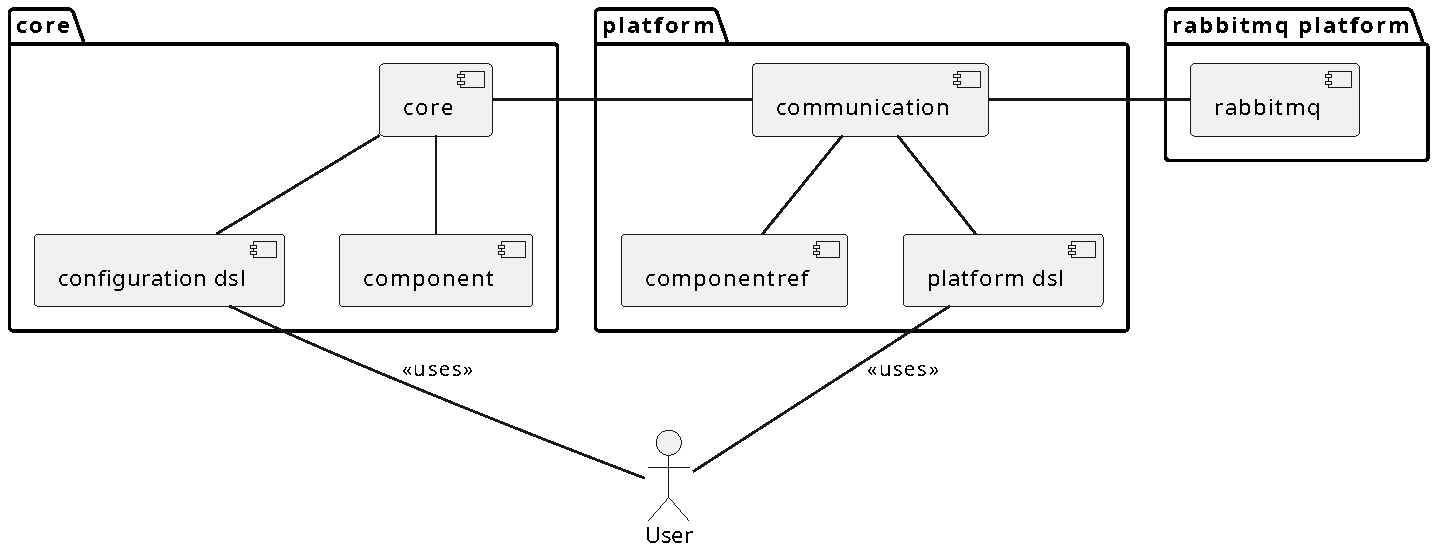
\includegraphics[width=\textwidth]{figures/package-diagram.pdf}
	\caption{Package diagram showing the modules that constitute the framework and their relationship.}
	\label{fig:package-diagram}
\end{figure}

In the~\Cref{tab:framework-modules} are reported a synthetic representation of the modules that constitute the framework with a corresponding
description.

\begin{table}
	\begin{tabularx}{\textwidth}{l X}
		\toprule
		\textbf{Module}            & \textbf{Description}                                                                                             \\ \midrule
		\texttt{Core}              & Defines all the pulverization concepts, exposing them as interfaces.
		Provides a DSL to specify the device types.                                                                                                   \\
		\texttt{Platform}          & Is responsible for executing all the device's components on the available infrastructure.
		Provides a DSL to configure the platform specifying which components should be used.                                                          \\
		\texttt{RabbitMQ Platform} & Represents a possible implementation for enabling intra-component communication leveraging RabbitMQ as protocol. \\ \bottomrule
	\end{tabularx}
	\caption{A tabular representation of the modules that constitute the framework.}
	\label{tab:framework-modules}
\end{table}

The pulverization framework relies on a three-level architecture. Each level of the framework's architecture is designed to use the functionalities
of the layer above and makes accessible their functionalities to the layer below.

The described architecture takes with it the implicit ``one-way dependency'' where the layer below depends on the layer above and not vice versa.
The~\Cref{fig:framework-architecture} depicts the architecture's choice made to design and build the framework.

\begin{figure}
	\centering
	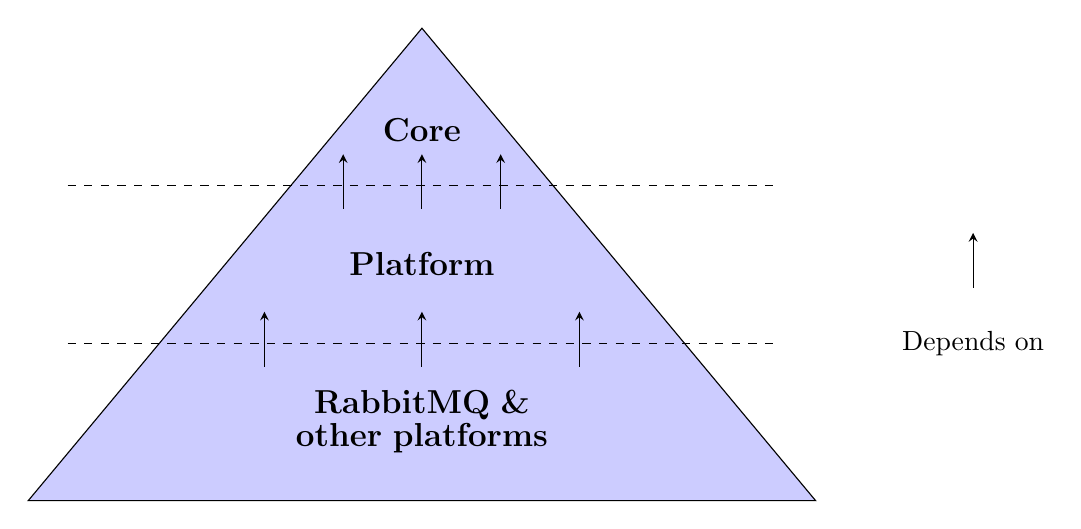
\begin{tikzpicture}
		\tikzstyle{fontbf} = [rectangle,text width=5cm,text centered,font=\bfseries]
		\draw[fill=blue!20] (0,0) -- (-5, -6) -- (5, -6) -- cycle;
		\draw[dashed] (-4.5,-2) -- (4.5,-2);
		\draw[dashed] (-4.5,-4) -- (4.5,-4);
		\draw[stealth-](0,-1.6) -- (0,-2.3);
		\draw[stealth-](-1,-1.6) -- (-1,-2.3);
		\draw[stealth-](1,-1.6) -- (1,-2.3);

		\draw[stealth-](0,-3.6) -- (0,-4.3);
		\draw[stealth-](-2,-3.6) -- (-2,-4.3);
		\draw[stealth-](2,-3.6) -- (2,-4.3);

		\draw[stealth-](7,-2.6) -- (7,-3.3);
		\node at (7,-4) {Depends on};

		\node[fontbf] at (0, -1.3) {\large Core};
		\node[fontbf] at (0, -3) {\large Platform};
		\node[fontbf] at (0, -5) {\large RabbitMQ \& other platforms};
	\end{tikzpicture}
	\caption{Architectural diagram showing how the pulverization framework is designed.}
	\label{fig:framework-architecture}
\end{figure}

Since this is a framework, it will likely be used by several users; therefore, it is strategic to minimize the cognitive effort that the user will
have to make to use it.

For a framework to be successful and usable, it must be able to provide an incremental approach to its use,
meaning that it must provide only the abstractions necessary for its use while at the same time providing clarity in its innermost components so that
the user can understand how it works and possibly extend the framework with external modules.

The ``pyramid architecture'' used by the framework tries to apply the concept described above (\Cref{fig:pyramid-user-knowledge}):
the tip of the pyramid represents the components' abstraction defined by the pulverization and those components are used and built by the user.
Those abstraction needs to be as clear as possible from a software engineering perspective.
As you move down the pyramid, the complexity of the modules increases but the user's knowledge of them decreases.

\begin{figure}
	\centering
	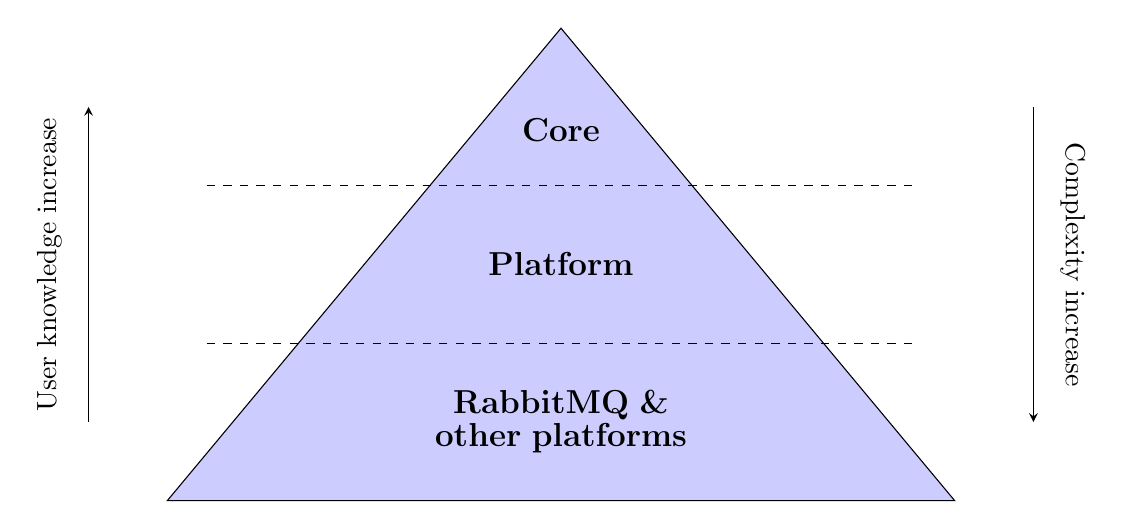
\begin{tikzpicture}
		\tikzstyle{fontbf} = [rectangle,text width=5cm,text centered,font=\bfseries]
		\draw[fill=blue!20] (0,0) -- (-5, -6) -- (5, -6) -- cycle;
		\draw[dashed] (-4.5,-2) -- (4.5,-2);
		\draw[dashed] (-4.5,-4) -- (4.5,-4);
		\draw [-stealth](6,-1) -- (6,-5);
		\draw [stealth-](-6,-1) -- (-6,-5);
		\node[rotate=-90] at (6.5,-3) {Complexity increase};
		\node[rotate=90] at (-6.5,-3) {User knowledge increase};
		\node[fontbf] at (0, -1.3) {\large Core};
		\node[fontbf] at (0, -3) {\large Platform};
		\node[fontbf] at (0, -5) {\large RabbitMQ \& other platforms};
	\end{tikzpicture}
	\caption{A correlation between the framework's complexity and the required user's knowledge to use the framework.}
	\label{fig:pyramid-user-knowledge}
\end{figure}

By designing the framework in this way, we open up different usage scenarios such as a basic use that requires only an understanding of the
basic concepts, to advanced uses that require a deep understanding of the framework enabling its complete usage and extension.

\todo{valutare se espandere qui con esempi o altro}

The sections below will describe the architectural choices made for each framework's module.

\subsection{Core module}
\label{sec:core-module}

Architecturally, the \emph{core} module is rather simple. Its simplicity is a consequence of the fact that this module is the main entry point
for the user, and the lower the complexity of this module, the faster the user can become familiar with the framework.
Moreover, a correct design of the interfaces defined in the \emph{core} module is a crucial aspect to consider to be aligned with the
pulverization concepts illustrated in the article~\cite{fi12110203}.

The pulverization represents a device as the combination of five components: \textbf{state}, \textbf{behaviour}, \textbf{communication},
\textbf{sensors} and \textbf{actuators}~\cite{fi12110203}.
All of those concepts are modeled by the framework through interfaces that the user will implement based on the specific scenario.

\begin{figure}
	\centering
	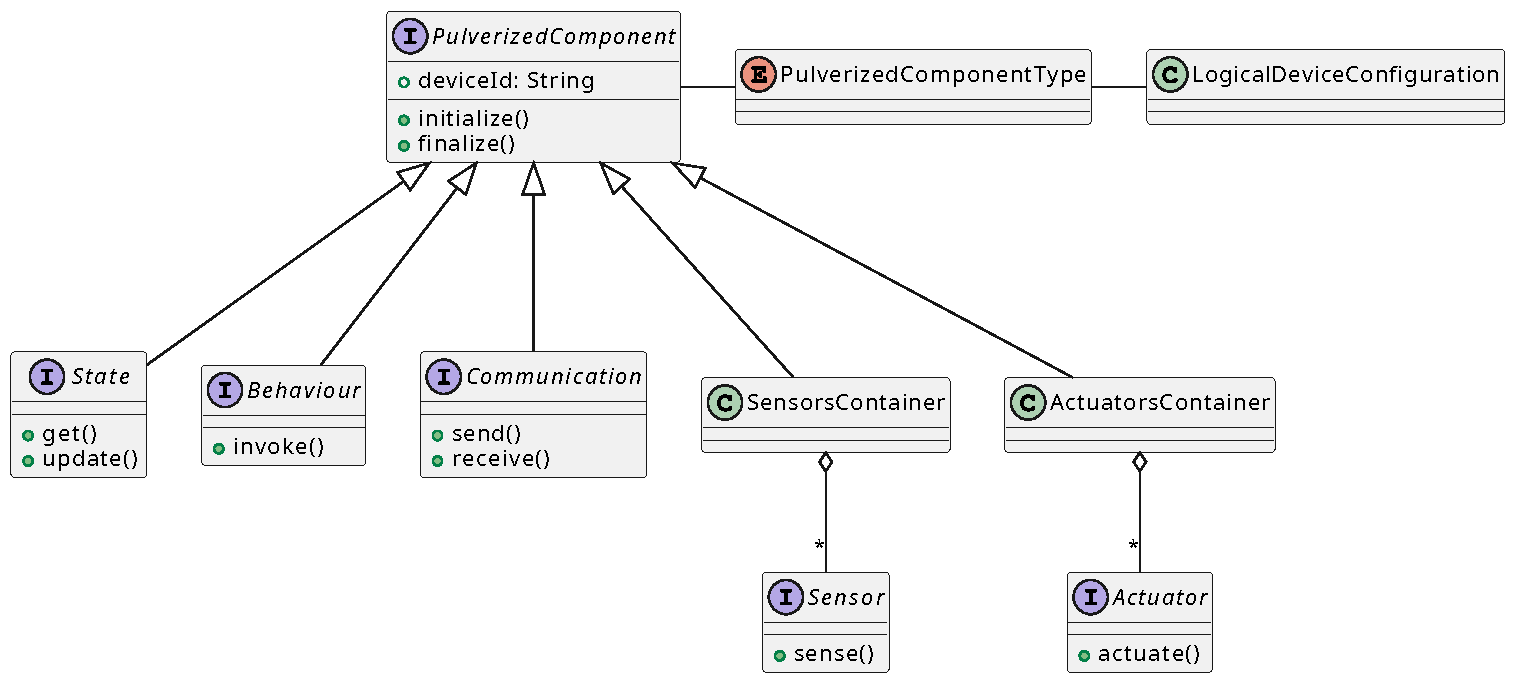
\includegraphics[width=\textwidth]{figures/core-design-interfaces.pdf}
	\caption{Class diagram showing the interfaces defined by the core module.}
	\label{fig:core-module-architecture}
\end{figure}

The~\Cref{fig:core-module-architecture} shows the concepts defined by the core module and their relationship.

This module provides a DSL to generate the configuration needed for the platform to run. In particular, the DSL provides a simple, clean and handy
way to create in a declarative fashion how many logical devices should the platform manage, and how those devices are made.

\subsection{Platform module}
\label{sec:platform-module}

The platform module defines the enabling concepts for system execution like intra-component communication and provides an abstraction for
representing a remote component and how to reach it; finally, it manages all the machinery needed to run the system.

The highly distributed nature of the pulverization has forced the design phase to abstract from the actual place where components are actually
deployed; in this way, we avoid the need for the user to specify and/or manage specific aspects of deployment but can focus solely on
application logic while remaining adherent to the objectives of the pulverization, which among many want to separate aspects of
deployment from aspects of application logic~\cite{fi12110203}.

Although the abstractions defined in this module are fundamental to the execution of the system, their understanding by the user is not essential.
Nevertheless, their understanding becomes crucial when the user wants to extend the framework with new features, like implementing a new protocol to
enable intra-communication components.

As said before, communication between components is a fundamental aspect to consider; for this reason, the \emph{communicator} concept comes in.
The communicator abstracts the way how the communication between two (pulverized) components occurs, defining how two components communicate with
each other. The design of this component abstracts from the message format and the type of the involved components, effectively making the
communicator highly generic and delegating all those complexities to the platform.

Finally, the platform module provides a DSL to allow the user to instantiate the platform and then actually run the system.
The DSL allows, declaratively, to specify the components intended to be executed in that specific deployment unit, as well as indicate which
specific communicator implementation to use. In~\Cref{fig:platform-module-architecture} is depicted the overall architecture of the platform module.

\begin{figure}
	\centering
	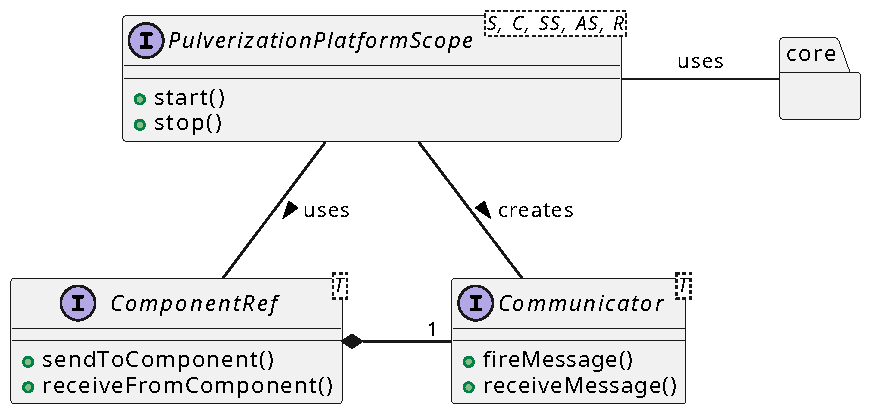
\includegraphics[width=0.8\textwidth]{figures/platform-design-interfaces.pdf}
	\caption{Class diagram showing the interfaces defined by the platform module.}
	\label{fig:platform-module-architecture}
\end{figure}

\subsection{Rabbitmq-platform module}
\label{sec:rabbitmq-platform-module}

This module implements a possible communicator that bases its operation on RabbitMQ. Although this module, at the time of writing, represents
the only implementation of a communicator, this does not mean that it should be the only possible solution.
Other communicators based on different technologies and infrastructures will likely be implemented in the future.

In this module, all the communication aspects that will be used for communication between components of the pulverized system are defined.
The design of the framework delegates to these types of implementations to handle low-level aspects like connections, retry on failure and so on.

While this module (or this kind of module more generally) requires a very good understanding of the concepts defined in
section~\ref{sec:platform-module} to be implemented, it requires no cognitive effort on the part of the user to be used.
\todo{Forward reference alla sezione dove si spiegano i dettagli implementativi di questo modulo}

% - New section ---------------------------------------------------------------

\section{Data flow in the framework}
\label{sec:framework-data-flow}

Pulverization based its design on the communication between components to create a synergy that allows the system to work properly.
The ``fragmentation'' of the devices into components allows the system to work independently from the specific deployment, focusing entirely on
the business logic of the application.
Is the responsibility of the framework to take care of the communication between components, and define how those communications should be handled.

The following sections will describe the data flow in the framework, from the point of view of the components and the point of the device.

\subsection{Components interaction}
\label{sec:framework-components-interaction}

The original formulation of the pulverization defines the component's interaction as follows (see~\Cref{fig:framework-components-interaction}):

\begin{figure}
	\centering
	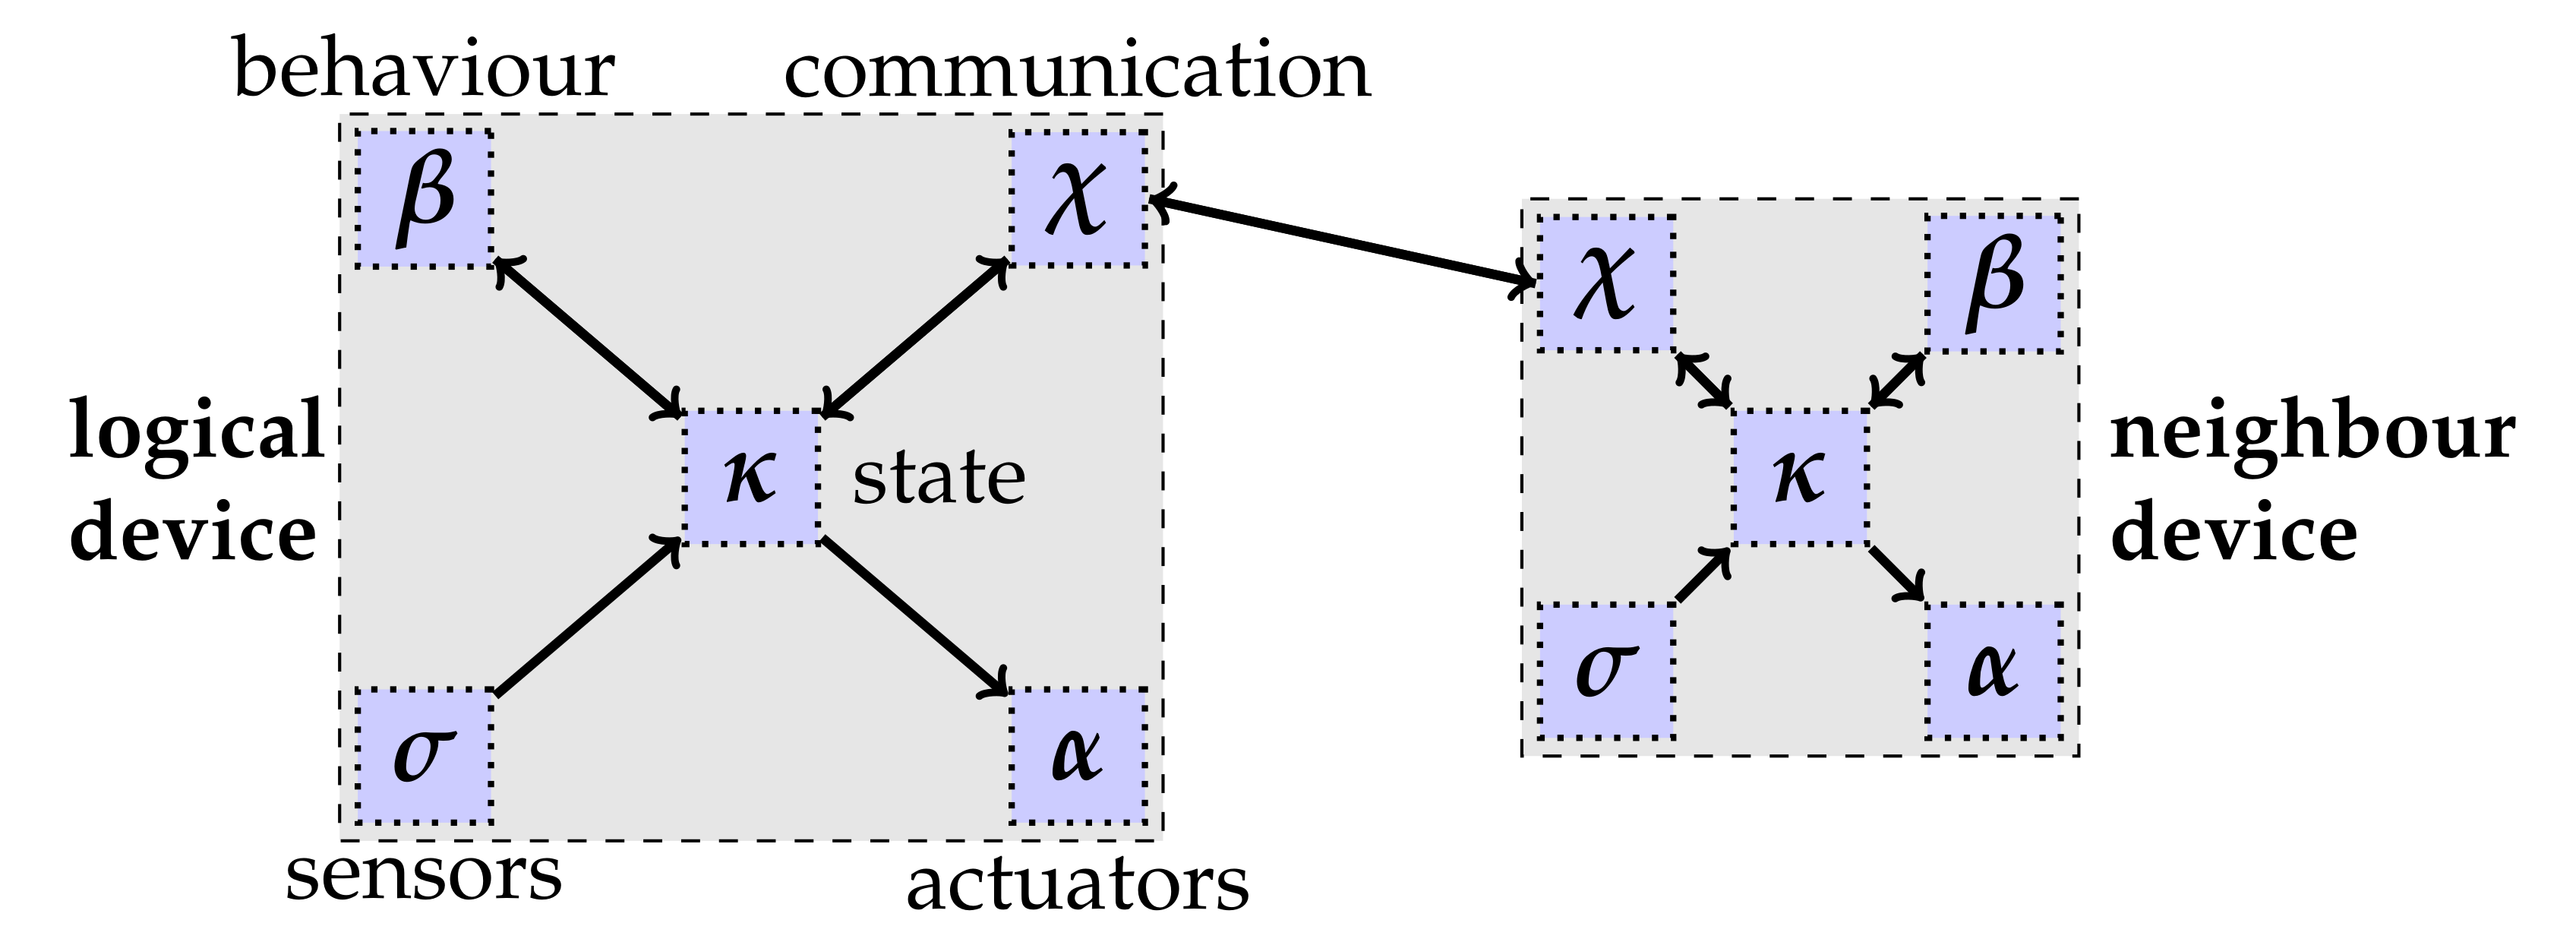
\includegraphics[width=\textwidth]{figures/original-components-interactions.png}
	\caption{Design of the interactions between components proposed in the original article~\cite{fi12110203}.}
	\label{fig:framework-components-interaction}
\end{figure}

Four interactions are involved in pulverization:
\begin{itemize}
	\item \textbf{Behaviour} to \textbf{State}: the \textbf{Behaviour} read from the \textbf{State} the \textit{sensed values}, the \textit
	      {communications} and the current \textit{state}, then update the \textbf{State} with information like \textit{new communication} to send to
	      all the neighbours, a set of \textit{prescriptive actions} to perform and the \textit{new state}.
	\item \textbf{Sensors} to \textbf{State}: the \textbf{Sensors} send to the \textbf{State} a set of \textit{sensed values}.
	\item \textbf{Actuators} to \textbf{State}: the \textbf{Actuators} receives from the \textbf{State} a set of \textit{prescriptive actions} to
	      perform.
	\item \textbf{State} to \textbf{Communicator}: the \textbf{State} sends to the \textbf{Communication} a \textit{new communication}
	      to send to all the neighbours and correspondingly the \textbf{Communication} send to the state all the \textit{communications} from the
	      neighbours.
\end{itemize}

\todo{Spiegare che la formulazione originale e' stata concepita come "nastro di turing" rappresentato dallo stato}

Despite this formulation being very clear and reasonable, it requires some extra communication to achieve the result.
For example, when the \textbf{Behaviour} component computes the \textit{new communication} to send to all the neighbours, it needs to send it to the
\textbf{State} component, which will then send it to the \textbf{Communicator} component. This not represents a problem per se but forces an extra
step to complete the communication, resulting in a possible inefficient communication pattern.

This kind of ``extra communication'' can be observed also in other component's interactions, like the one between the \textbf{Sensors} and the
\textbf{Behaviour} and the \textbf{Actuators} and the \textbf{Behaviour}. In all of those cases, the \textbf{State} component is involved in the
communication creating an extra step.

The framework uses a different formulation of the component's interaction to reduce the extra communication simplifying the overall communication
pattern. This formulation is depicted in~\Cref{fig:framework-components-interaction-2}.

\begin{figure}
	\centering
	\missingfigure[figwidth=\textwidth]{Create a diagram showing the interaction between components defined in the framework}
	\caption{Interaction between components.}
	\label{fig:framework-components-interaction-2}
\end{figure}

This new formulation is based on the fact that the \textbf{behaviour} component has a direct dependency on all the other four components,
in this way, the \textbf{behaviour} component can directly interact with the other components without the need to be intermediated by the
\textbf{State} component.

The component's interaction is now defined as follows:
\begin{itemize}
	\item \textbf{Sensors} to \textbf{Behaviour:} the \textbf{Sensors} send to the \textbf{Behaviour} a set of \textit{sensed values}.
	\item \textbf{Actuators} to \textbf{Behaviour:} the \textbf{Actuators} receives from the \textbf{Behaviour} a set of \textit{prescriptive
		      actions} to perform.
	\item \textbf{Communication} to \textbf{Behaviour:} the \textbf{Communication} sends to the \textbf{Behaviour} a set of \textit{communications}
	      from the neighbours and receives from the \textbf{Behaviour} the \textit{new communication} for the neighbours.
	      \item\textbf{State} to \textbf{Behaviour:} the \textbf{Behaviour} read from the \textbf{State} the \textit{current state} and write to it
	      the \textit{new state}.
\end{itemize}

Now, the \textbf{Behaviour} component is central in the communication between components, and it is the only component that needs to interact with all the other components.

Below, is presented a formal description of each component's interaction with the \textbf{Behaviour} component.

For what concern the \textbf{Sensors} and \textbf{Actuators} components, the interaction with the \textbf{Behaviour} component is specular: the
sensors send to the behaviour the sensed values and the actuators receive from the behaviour the prescriptive actions to perform.
The sequence diagrams in~\Cref{fig:framework-components-interaction-2-sensors-actuators} show the interaction of the sensors and actuator with the
behaviour.

\begin{figure}
	\centering
	\missingfigure[figwidth=\textwidth]{Create a sequence diagram showing the interaction between sensors and actuators with the behaviour}
	\caption{Interaction between sensors and actuators with the behaviour.}
	\label{fig:framework-components-interaction-2-sensors-actuators}
\end{figure}

The \textbf{Communication} and \textbf{Behaviour} interaction is bidirectional, which means that the communication sends to the behaviour all the
messages coming from the neighbours and the behaviour sends to the communication component the new messages that should be propagated
to the neighbours.
Reasoning on the way this interaction occurs could lead to modeling it using a specific pattern (e.g. synchronous or asynchronous) but is fundamental
to abstract over the specific pattern giving the freedom to use the one that better fits the current situation.
The sequence diagrams in~\Cref{fig:framework-components-interaction-2-communication-behaviour} shows the interaction between the communication and
behaviour components using a communication pattern which not represents the only possible one.

\begin{figure}
	\centering
	\missingfigure[figwidth=\textwidth]{Create a sequence diagram showing the interaction between communication and behaviour}
	\caption{Interaction between communication and behaviour.}
	\label{fig:framework-components-interaction-2-communication-behaviour}
\end{figure}

Even the \textbf{State} and \textbf{Behaviour} interaction is bidirectional.
The behaviour queries the state component to get the current state, then, the behaviour computes the new state and writes it to the state component.
Even in this case, the way this interaction is modeled is not fundamental and should be abstracted over the specific pattern.
The sequence diagrams in~\Cref{fig:framework-components-interaction-2-state-behaviour} shows the interaction between the state and behaviour.

\begin{figure}
	\centering
	\missingfigure[figwidth=\textwidth]{Create a sequence diagram showing the interaction between state and behaviour}
	\caption{Interaction between state and behaviour.}
	\label{fig:framework-components-interaction-2-state-behaviour}
\end{figure}

\subsection{Device cycle}
\label{sec:framework-device-cycle}

In the previous section, we looked at what interactions there are between the various components. In this section, we analyze how these interactions
are synchronized to ensure the overall operation of the device.

By device cycle, we mean the sequence of operations that the device must perform to function. In the context of pulverization, this cycle is
pre-determined and well-structured.

The cycle consists of the following steps:

\begin{itemize}
	\item \emph{Context acquisition:} the device retrieves information from sensors and communications.
	\item \emph{Computation:} the behaviour function is applied using the state, sensors and communications, producing an output.
	\item \emph{Coordination:} the coordination data is sent to all the neighbours.
	\item \emph{Actuation:} the actuators are activated to execute the prescriptive actions produced by the behaviour.
\end{itemize}

Given the highly distributed nature of pulverization, it is quite complex to manage this cycle properly. For this reason, it is left to the platform
to manage any synchronization and controls to ensure that the cycle runs smoothly.

To deal with this problem, a model was created that abstracts from where the various components are deployed, thus creating a uniform level
to access the components while delegating to the platform the logic on how to reach the component ``physically''. In this way it is also possible
to make optimizations on communications, e.g., if two components belong to the same deployment unit, then they communicate directly in memory,
otherwise, they take advantage of one of the provided implementations to communicate over the network.

The modeling provided for this problem involves the use of two concepts: the \emph{ComponentRef} and the \emph{Communicator}.
The former embodies the concept of ``reference to a component'' abstracting from where the component is physically deployed. In this way, the
communication with another component can be done seamlessly and clearly.
The latter is used by the \emph{ComponentRef} to communicate with the component it refers to. The \emph{Communicator} manages all the low level
aspects of the communication, e.g., the protocol used to communicate, the serialization of the data, etc.

Is the responsibility of the platform to create the right \emph{Communicator} for each \emph{ComponentRef} based on the initial configuration given
by the user. Separating the reference to a component from how the communication occurs, allows the platform to optimize all the communication and change in real-time the communicator based, for example, on the new deployment.

% \todo{definire una sezione per valutare l'approccio asincrono dello scambio dati}

% \section{Framework dynamics}
% \label{sec:framework-dynamics}

% The pulverization framework is designed to adapt its behaviour based on specific configurations without the need for the user to change the
% business logic. This section will describe from a high-level perspective how the framework adapts its behaviour based on the configuration.

% One fundamental aspect of pulverization is the ability to ``move'' the component of a device from one location to another in a transparent way.

% The pulverization framework is designed to be able to take each one of the five components and set up the deployment to match the current
% configuration. The framework force the user to define the components by reasoning in terms of relations between itself and the other components,
% in this way, we isolate the single logic of the component and we can easily move it to another deployment unit if needed.
% Moreover, by defining in this way the components, the framework can easily determine if the other component is remote or in the same deployment unit,
% optimizing the communication between them.

% \begin{figure}[h]
%     \centering
%     \missingfigure[figwidth=\textwidth]{a diagram showing how easy is to move components into another deployment unit.}
%     \caption{The relation between the components of a device and the deployment unit.}
%     \label{fig:framework-dynamics}
% \end{figure}

% This feature is fundamental to cover different scenarios and contexts where a dynamic adaptation of the system is needed. For example, considering
% the case of a smart device, the system can decide to move the \emph{behaviour} from the device to a cloud service because of low batter or any other
% issues, in this way the heavy computation can be offloaded to a more powerful machine so that the device can continue to run for a longer time
% managing only aspects of sensing and actuation.

% The \Cref{fig:dynamics-example} depicts a possible scenario where the \emph{behaviour} is moved from the device to a cloud service, depending on
% the current context.
% \begin{figure}
%     \centering
%     \missingfigure[figwidth=\textwidth]{a diagram showing the example above.}
%     \caption{}
%     \label{fig:dynamics-example}
% \end{figure}

% To achieve this dynamic feature, the framework works based on two perspectives of a single component:
% \begin{itemize}
%     \item \textbf{Component implemented logic} (behaviour of the component)
%     \item \textbf{Component communication logic} (how the component communicates with the other components)
% \end{itemize}

% The first perspective is the one that the user will implement, describing and implementing the logic of the component.
% The second perspective is the one that the framework will use to determine how the communication between the components should be handled.
% Generally, the communication logic could be pre-defined by the framework, but the user can override it if needed.
% In this way, we enable full customization of the framework giving the user the ability to define how the communication between components should
% occur, or use the default implementation.

% \begin{figure}[h]
%     \centering
%     \missingfigure[figwidth=\textwidth]{a diagram showing the two perspectives of a component.}
%     \caption{}
%     \label{fig:component-perspectives}
% \end{figure}

% The~\Cref{fig:component-perspectives} shows the two perspectives of a component, the one implemented by the user and the one used by the framework.
% \todo{rileggere la sezione e vedere se ridurre il livello di dettaglio oppure introdurre nuovi concetti}
